\chapter{Approach}
\label{ch:approach}
As has been discussed in chapter \ref{ch:related}, there is a need for a tool to detect as much as possible syntax errors in RDF documents. As a result to this need, this study was held and this chapter will cover the approach used in the proposed solution.

\section{ANTLR: The Core Component}
In order to find a parser which can accept the error production rules in its grammar, our choice was to use ANTLR framework to automatically generate the required parser. Lots of features in ANTLR motivate us to use it in the proposed solution, such as: 1) its grammar can equip with error production rules and when a couple of tokens match such rules, the parser will fire  error notifications, 2) it uses a parse tree to parse input token and the view of this parse tree can be delivered as an output to the user at the end of parsing process, it supports the auto-generation of parsers in different programming language, as it was discussed in Chapter \ref{ch:preliminaries}.
\section{Overview of the Proposed Solution}

 To represent the approach in more clear way, {\it figure \ref{Fig:Approach}} was invented. It shows the technique used to handle an RDF text, having some syntax errors. follows are the sequence steps which highlight the main milestones of this approach:
 \begin{enumerate}[label=(\alph*)]
\item \textbf{Reading RDF text}: a ordinary RDF file is submitted to our application. The application starts with reading the file. In case of large files, it is going to be splitted into two or more chunks based on the volume of the file. each chunk will be processed separately from others.  {\it Figure \ref{Fig:Approach}}(a) demonstrates this part. 
\item \textbf{Detection of syntax errors}: the parser has predefined rules for syntax errors, once a rule is matched with a sequence of input tokens, it stores this error to be reported later in the error report. Reading of input tokens continues till the end of the file while searching for matches for syntax errors. In  {\it figure \ref{Fig:Approach}}(b) lines surrounded with red color simulate detected lines which contain syntax errors. 
\item \textbf {Healing some of detected errors}: this feature firstly needs to be selected by the user to be active. The method of healing syntax errors focuses of a certain type of errors which has only one predefined solution in standards. Those errors like missing of dot at the end of triple, missing semi-colon after multiple predicates sharing same subject, missing comma after multiple objects having same subject and predicate. Lines surrounded with green color in {\it figure \ref{Fig:Approach}}(c) represents some of healed lines from error at the end of the correction phase.  
\item\textbf {Generation of output text}: In this example, it is previously assumed that the user selected to correct found errors.  {\it Figure \ref{Fig:Approach}}(d) describes how the output should look like. It is sufficiently clear that healed lines are not shown, but some of unhealed line are still showing up. This comes as a normal result of existing of syntax errors which can have multiple solution, for example, a literal with multiple language tags like "me"@en@de. also it could be that the healing term is unknown, for example, missing of a prefix declaration for a certain local name-space. 
\end{enumerate} 

\begin{figure}
	\centering
	  	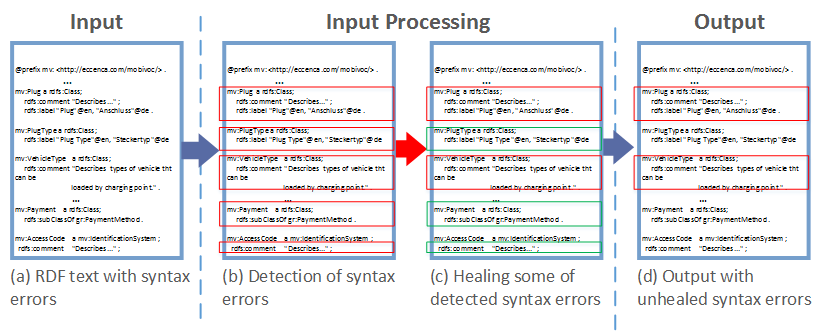
\includegraphics[width=1\textwidth]{images/Approach.png}
		\caption{\textbf{Overview of the proposed solution}}
		\label{Fig:Approach}  
\end{figure}
\section{Representation in Pseudo-code}
To functionally represent the approach of this study, Algorithm \ref{alg:algorithm-main} was engineered. It is showing the abstract behaviour of the developed program where \textbf{syntaxRules} variable combines both correct syntax rules and incorrect ones. A \textbf{While loop} traverse till the end of the file or a single chunk if a large file was separated in a couple of chunks. The \textbf{tokensToBeMatched}  variable collected a sequence of followed tokens to be matched either with correct or incorrect syntax rules.

More importantly is the syntax errors finding, for that reason \textbf{tokensToBeMatched} is checked if its content are drawn by \textbf{incorrectSyntaxRules}, if it falls in that situation, then the content of \textbf{tokensToBeMatched} is considered as a syntax error and the parser sends a notification for those listener APIs  whose are interesting of further processing of the error. 

\begin{algorithm}[H] 
 \caption{Representation of the proposed solution  in pseudo-code}
 \label{alg:algorithm-main}
 \KwData{inputText, correctSyntaxRules, incorrectSyntaxRules, CorrectionIsSelected}
 \KwResult{foundSyntaxErrors and recoveredSyntaxErrors}

% S = subject(M)\;
foundSyntaxErrors = [ ];\\
recoveredSyntaxErrors = [ ];\\
$syntaxRules \leftarrow correctSyntaxRules + incorrectSyntaxRules;$\\
		\While{token in inputText \&\& $inputText \neq EOF$}{
tokenToBeMatched += token;\\
		\uIf{ syntaxRules contains tokensToBeMatched}{
		\uIf{ incorrectSyntaxRules contains tokensToBeMatched}{
		 foundSyntaxErrors.push(tokensToBeMatched);\\
		\uIf{ CorrectionIsSelected}{
		\uIf{ canErrorRecovered(tokensToBeMatched)}{
		  \uIf{recoverSyntaxError(tokensToBeMatched)}{
		  recoveredSyntaxErrors.push(tokensToBeMatched);\\
		  foundSyntaxErrors.pop(tokensToBeMatched);\\

		  }
		}
		}
		}
		 $tokensToBeMatched \leftarrow ""$  \\
		 $token \leftarrow ""$  	\\	
		}
}
return foundSyntaxErrors , recoveredSyntaxErrors
\end{algorithm}

The correction of error is a feature that can be activated with the user options. In case, the user selects to enable it, then the Error Correction Module will traverse all list of detected syntax errors and based on the error message, it can identify if the error can be corrected or goes with correction. At the end of the correction phase, a report of the corrected error will be delivered to the user. 

\section{Categorization of RDF Syntax Errors}
 In this approach, Turtle\footnote{\href{https://www.w3.org/TR/turtle/}{Turtle}} and N-Triples\footnote{\href{https://www.w3.org/TR/n-triples/}{N-Triples}} RDF serializations were the core syntaxes in our study, as a use case. Additionally, Turtle is a special case of N-Triples. for this reason, the grammar of the proposed solution was created based on Turtle format. 
 
 Furthermore, since the significant part in this study is the ability to identify syntax errors, the expected syntax errors need to be known to be injected in the grammar. \cite{TurtleTests:Online} plays an important role in syntax errors declaration. It contains several files of Turtle format to show both correct and incorrect syntaxes and it is supposed to be used to validate any parser that parses Turtle format, if it can recognized a incorrect syntax as an incorrect and vice verse . 
 
 In table \ref{tab:syntaxErrorCate}, we have categorized the syntax errors (found in the files at \cite{TurtleTests:Online}) into multiple groups. Each of those files can be identified if a file represents a correct syntax or incorrect one based on it title if it contains the workd "Bad" which means it contains an incorrect syntax, then, it can be syntactically engineered in our grammar.  
 

\newcounter{cA} 
\setcounter{cA}{1}
\begin{longtable}{|c|c|c|l|l}
    \caption{Categorization of syntax errors }
    \label{tab:syntaxErrorCate}

    \centering

\cline{2-5}
Sn. & Catergory & Position & Sample &  \\ \midrule 
\thecA     \addtocounter{cA}{1}  & \multirow{3}{*}{ \textcolor{blue}{Bad String Escape}
} & Literal & \textcolor{red}{"a\textbackslash zb" } &  \\ \cline{1-1} \cline{3-4}
\thecA     \addtocounter{cA}{1}  &  & Literal & \textcolor{red}{"\textbackslash uWXYZ"}  &  \\ \cline{1-1} \cline{3-4}
\thecA     \addtocounter{cA}{1}  &  & Literal &  \textcolor{red}{"\textbackslash U0000WXYZ"} &  \\   \midrule \midrule
\thecA     \addtocounter{cA}{1}  &  \multirow{5}{*}{ \textcolor{blue}{Missuse of Keywords}} & Predicate &  :s \textcolor{red}{ A} :o . &  \\   \cline{1-1} \cline{3-4}
\thecA     \addtocounter{cA}{1} &  & Subject &\textcolor{red}{ a} :p :o . &  \\ \cline{1-1} \cline{3-4}
\thecA     \addtocounter{cA}{1} &  & Object & :s :p \textcolor{red}{ a} .  &  \\ \cline{1-1} \cline{3-4}
\thecA     \addtocounter{cA}{1} &  & Subject & \textcolor{red}{true} :p :o . &  \\ \cline{1-1} \cline{3-4}
\thecA     \addtocounter{cA}{1}  &  & Object & :s \textcolor{red}{true} :o . &  \\   \midrule \midrule
\thecA     \addtocounter{cA}{1}  &   \textcolor{blue}{Bad Language Tag} & Language Tag &  “duck”@\textcolor{red}{1} &  \\ \midrule \midrule
\thecA     \addtocounter{cA}{1}  &  \multirow{5}{*}{ \textcolor{blue}{Bad Local Namespace in Prefixed IRI}} & Prefixed IRI &  :s :p \textcolor{red}{ :-a}  . &  \\   \cline{1-1} \cline{3-4}
\thecA     \addtocounter{cA}{1}  &  & Prefixed IRI & :s :p \textcolor{red}{ :o\%2} .&  \\ \cline{1-1} \cline{3-4}
\thecA     \addtocounter{cA}{1}  &  & Prefixed IRI & :s :p \textcolor{red}{ :\%o2} .&  \\ \cline{1-1} \cline{3-4}
\thecA     \addtocounter{cA}{1}  &  & Prefixed IRI & :s :p \textcolor{red}{:a\texttt{\~{}}b} . &  \\ \cline{1-1} \cline{3-4}
\thecA     \addtocounter{cA}{1}  &  & Prefixed IRI &  \textcolor{red}{:a\textbackslash u0039} :p :o . &  \\   \midrule \midrule
\thecA     \addtocounter{cA}{1}  & \multirow{2}{*}{ \textcolor{blue}{Bad Prefix Label in  Prefixed IRI}
} & Prefixed IRI & :s :p \textcolor{red}{ ex.}:o . &  \\ \cline{1-1} \cline{3-4}
\thecA     \addtocounter{cA}{1}  &  & Prefixed IRI & :s :p \textcolor{red}{.ex}:o .  &  \\ \midrule \midrule
\thecA     \addtocounter{cA}{1}  &  \multirow{18}{*}{ \textcolor{blue}{Bad Syntax from N3 Notation }} & Curly Brackets & \textcolor{red}{ \{ :a :q :c . \}}  :p :o . &  \\   \cline{1-1} \cline{3-4}
\thecA     \addtocounter{cA}{1}  &  & Equal Sign & :a \textcolor{red}{ =} :b .&  \\ \cline{1-1} \cline{3-4}
\thecA     \addtocounter{cA}{1}  &  & N3 Paths & \textcolor{red}{ :x.
  ns:p.
    ns:q } :p :z . &  \\ \cline{1-1} \cline{3-4}
\thecA     \addtocounter{cA}{1}  &  & N3 Paths & \textcolor{red}{:x\textasciicircum ns:p } :p :z . &  \\ \cline{1-1} \cline{3-4}
\thecA     \addtocounter{cA}{1}  &  & ‘is .. of’  & :z \textcolor{red}{ is}  :p \textcolor{red}{ of}  :x . \\  & & Pattern &  &  \\ \cline{1-1} \cline{3-4}
\thecA     \addtocounter{cA}{1}  &  & DOTs without  &\textcolor{red}{ :a.:b.:c } . \\ & & Space & &  \\ \cline{1-1} \cline{3-4}
\thecA     \addtocounter{cA}{1}  &  & '@keywords' & \textcolor{red}{@keywords  
} a . \\ & & Pattern & x a Item . &  \\\cline{1-1} \cline{3-4}
\thecA     \addtocounter{cA}{1}  &  & '@keywords' & \textcolor{red}{@keywords  
}  . \\ & & Pattern & 
x \textcolor{red}{@a} Item .  &  \\ \cline{1-1} \cline{3-4}  \\  
\thecA     \addtocounter{cA}{1}  &  & '\textless=' Pattern & :s \textcolor{red}{ \textless=} :o .&  \\ \cline{1-1} \cline{3-4}
\thecA     \addtocounter{cA}{1}  &  & '=\textgreater' Pattern  & :s   \textcolor{red}{ =\textgreater} :o  .&  \\ \cline{1-1} \cline{3-4}
\thecA     \addtocounter{cA}{1}  &  & '@forSome' & \textcolor{red}{@forSome } :x . \\ & & Pattern & &  \\ \cline{1-1} \cline{3-4}
\thecA     \addtocounter{cA}{1}  &  & '@forAll' & \textcolor{red}{@forAll } :x . \\ & & Pattern & &  \\ \cline{1-1} \cline{3-4}
 \midrule \midrule
\thecA     \addtocounter{cA}{1}  & \multirow{4}{*}{ \textcolor{blue}{Bad Prefix Label in Directives}
} & \multirow{2}{*}{Directive} & @prefix  \textcolor{red}{eg.} :\textless example\textgreater . \\ & &  & \textcolor{red}{eg.}:s  :p  :o  . &  \\\cline{1-1} \cline{3-4}
\thecA     \addtocounter{cA}{1}  &   & \multirow{2}{*}{Directive} & @prefix   \textcolor{red}{.eg} :\textless example\textgreater . \\ & &  & \textcolor{red}{.eg}:s  :p  :o . &  \\\cline{1-1} \cline{3-4} \midrule \midrule
\thecA     \addtocounter{cA}{1}  &  \multirow{5}{*}{ \textcolor{blue}{Bad Number as a Literal:}} & Literal &  :s :p  \textcolor{red}{ 123.abc}  . &  \\   \cline{1-1} \cline{3-4}
\thecA     \addtocounter{cA}{1}  &  & Literal & :s :p \textcolor{red}{ 123e} .&  \\ \cline{1-1} \cline{3-4}
\thecA     \addtocounter{cA}{1}  &  & Literal & :s :p \textcolor{red}{ 123abc} .&  \\ \cline{1-1} \cline{3-4}
\thecA     \addtocounter{cA}{1}  &  & Literal & :s :p \textcolor{red}{0x123} . &  \\ \cline{1-1} \cline{3-4}
\thecA     \addtocounter{cA}{1}  &  & Literal & :s :p  \textcolor{red}{+- 1} . &  \\   \midrule \midrule
\thecA     \addtocounter{cA}{1}  &  \multirow{8}{*}{ \textcolor{blue}{Bad Directives}} &  \multirow{2}{*}{Directive} &  \textcolor{red}{\#Missing a prefix for ':'}\\
& & & \textcolor{red}{ :}s \textcolor{red}{ :}p  "x"  . &  \\   \cline{1-1} \cline{3-4}
 \thecA     \addtocounter{cA}{1}  &  & \multirow{2}{*}{Directive} &   \textcolor{red}{\#Missing an IRI}\\
& & & @prefix ex: . &  \\   \cline{1-1} \cline{3-4}
 \thecA     \addtocounter{cA}{1}  &  & \multirow{2}{*}{Directive} &   \textcolor{red}{\#Missing a prefix label}\\
& & &@prefix \textless example\textgreater . &  \\   \cline{1-1} \cline{3-4}
 \thecA     \addtocounter{cA}{1}  &  & \multirow{2}{*}{Directive} &   \textcolor{red}{\#Missing a colon }\\
& & & @prefix ex \textless example\textgreater . &  \\   \midrule \midrule
\thecA     \addtocounter{cA}{1}  &  \multirow{8}{*}{ \textcolor{blue}{Bad String}} & Literal &  :s :p \textcolor{red}{ "abc' }. &  \\   \cline{1-1} \cline{3-4}
\thecA     \addtocounter{cA}{1}  &  & Literal &  :s :p \textcolor{red}{'abc"  }. &  \\ \cline{1-1} \cline{3-4}
\thecA     \addtocounter{cA}{1}  &  & Literal &  :s :p \textcolor{red}{ '''abc' }.  &  \\ \cline{1-1} \cline{3-4}
\thecA     \addtocounter{cA}{1}  &  & Literal &  :s :p \textcolor{red}{ """abc'''  }. &  \\ \cline{1-1} \cline{3-4}
\thecA     \addtocounter{cA}{1}  &  & Literal &  :s :p \textcolor{red}{ """abc }. &  \\ \cline{1-1} \cline{3-4}
\thecA     \addtocounter{cA}{1}  &  & Literal &  :s :p \textcolor{red}{ """abc""""@en }. &  \\ \cline{1-1} \cline{3-4}
\thecA     \addtocounter{cA}{1}  &  & Literal &  :s :p \textcolor{red}{ '''abc''''@en} . &  \\ \cline{1-1} \cline{3-4}
\thecA     \addtocounter{cA}{1}  &  & Literal &  :s :p \textcolor{red}{ "abc"@en\textasciicircum \textasciicircum xsd:String }. &  \\   \midrule \midrule
\thecA     \addtocounter{cA}{1}  &  \multirow{5}{*}{ \textcolor{blue}{Bad Structure }} & Nquads & \multirow{2}{*}{\textcolor{red}{ \textless s\textgreater  \textless p\textgreater  \textless o\textgreater  \textless g\textgreater } . }\\ & &  Pattern &  \\   \cline{1-1} \cline{3-4}
\thecA     \addtocounter{cA}{1}  &  & Subject & \textcolor{red}{ “Hello”} :p :o .&  \\ \cline{1-1} \cline{3-4}
\thecA     \addtocounter{cA}{1}  &  & Predicate & :s \textcolor{red}{ “Hello”} :o .&  \\ \cline{1-1} \cline{3-4}
\thecA     \addtocounter{cA}{1}  &  & Predicate & :s \texttt{\textcolor{red}{[ ]}} :o . &  \\ \cline{1-1} \cline{3-4}
\thecA     \addtocounter{cA}{1}  &  & Predicate & :s \textcolor{red}{ \_:blank} :o .&  \\ \cline{1-1} \cline{3-4}
\thecA     \addtocounter{cA}{1}  &  & Triple &  \textcolor{red}{ \#Missing dot at the triple end} \\ & &  &  :s  :p  :o&  \\ \cline{1-1} \cline{3-4}
\thecA     \addtocounter{cA}{1}  &  & Triple & :s  :p  :o .\textcolor{red}{.. } &  \\ \cline{1-1} \cline{3-4}
\thecA     \addtocounter{cA}{1}  &  & Triple & :s   :p  :o \textcolor{red}{; } &  \\ \cline{1-1} \cline{3-4}
\thecA     \addtocounter{cA}{1}  &  & Triple &  \textcolor{red}{ \#Missing an object in a triple} \\ & &  & :s :p  .&    \\   \midrule \midrule
\thecA     \addtocounter{cA}{1}  &  \multirow{6}{*}{ \textcolor{blue}{Bad IRI:}} &  IRI & \textless
 http:// space\textgreater { a}  :o . &  \\   \cline{1-1} \cline{3-4}
\thecA     \addtocounter{cA}{1}  &  &  IRI &  \textless http://\textcolor{red}{\texttt{\textbackslash u00ZZ11}}\textgreater { :p}  :o .&  \\ \cline{1-1} \cline{3-4}
\thecA     \addtocounter{cA}{1}  &  &  IRI & \textless http://\textcolor{red}{\texttt{\textbackslash U00ZZ1111}}\textgreater { :p}  :o .&  \\ \cline{1-1} \cline{3-4}
\thecA     \addtocounter{cA}{1}  &  &  IRI & \textless http:// \\ &  &  & \textgreater { :p}  :o . &  \\ \cline{1-1} \cline{3-4}
\thecA     \addtocounter{cA}{1}  &  &  IRI &  \textless http://\textcolor{red}{\texttt{\textbackslash}}\textgreater { :p}  :o . &  \\   \midrule \midrule
\end{longtable}






 
